\documentclass[11pt,a4paper]{article}
\usepackage[utf8]{inputenc}
\usepackage{amsmath}
\usepackage{amsfonts}
\usepackage{amssymb}
\usepackage[pdftex]{graphicx}
\usepackage{float}
\setlength{\parindent}{0in}
\begin{document}
\tableofcontents
\newpage

\section{Report}
\label{sec-1}
\subsection{\textbf{DONE} Vision \& Business case}
\label{sec-1-1}

   \texttt{CLOSED:} \textit{2012-11-21 Wed 13:00}

\begin{itemize}
\item Introduction
\item Problem statement
\item Summary of system features
\end{itemize}
\subsection{\textbf{DONE} Use cases}
\label{sec-1-2}

   \texttt{CLOSED:} \textit{2012-12-16 Sun 01:34}
\subsubsection{\textbf{DONE} Use cases (text)}
\label{sec-1-2-1}

    \texttt{CLOSED:} \textit{2012-12-16 Sun 01:34}
\begin{itemize}

\item \textbf{DONE} UC1: Create new document\\
\label{sec-1-2-1-1}%
\texttt{CLOSED:} \textit{2012-11-21 Wed 13:00}


\item \textbf{DONE} UC2: Edit document\\
\label{sec-1-2-1-2}%
\texttt{CLOSED:} \textit{2012-11-21 Wed 13:00}


\item \textbf{DONE} UC3: Delete document\\
\label{sec-1-2-1-3}%
\texttt{CLOSED:} \textit{2012-11-22 Thu 11:45}


\item \textbf{DONE} UC4: Merging documents (resolve conflict)\\
\label{sec-1-2-1-4}%
\texttt{CLOSED:} \textit{2012-12-16 Sun 01:21}


\item \textbf{DONE} UC5: Offline sync\\
\label{sec-1-2-1-5}%
\texttt{CLOSED:} \textit{2012-11-22 Thu 11:45}


\item \textbf{DONE} UC6: New folder\\
\label{sec-1-2-1-6}%
\texttt{CLOSED:} \textit{2012-11-22 Thu 12:47}


\item \textbf{DONE} UC7: New project\\
\label{sec-1-2-1-7}%
\texttt{CLOSED:} \textit{2012-11-22 Thu 13:05}


\item \textbf{DONE} UC8: Find old version of document\\
\label{sec-1-2-1-8}%
\texttt{CLOSED:} \textit{2012-12-16 Sun 01:33}


\item \textbf{DONE} UC9: Share Document\\
\label{sec-1-2-1-9}%
\texttt{CLOSED:} \textit{2012-12-16 Sun 01:26}


\item \textbf{DONE} UC10: Log in\\
\label{sec-1-2-1-10}%
\texttt{CLOSED:} \textit{2012-12-16 Sun 01:27}

\end{itemize} % ends low level
\subsubsection{\textbf{DONE} Use Case Model (UML)}
\label{sec-1-2-2}

    \texttt{CLOSED:} \textit{2012-11-22 Thu 12:47}
\subsection{\textbf{DONE} Supplementary specification (FURPS+)}
\label{sec-1-3}

   \texttt{CLOSED:} \textit{2012-12-17 Mon 03:09}

\begin{itemize}
\item $\Box$ Functionality
\item $\Box$ Usability
\item $\Box$ Reliability
\item $\Box$ Performance
\item $\Box$ Supportability
\end{itemize}
\subsection{\textbf{DONE} Glossary}
\label{sec-1-4}

   \texttt{CLOSED:} \textit{2012-11-21 Wed 13:01}
\subsection{\textbf{DONE} System sequence diagram}
\label{sec-1-5}

   \texttt{CLOSED:} \textit{2012-11-22 Thu 12:05}
\subsection{\textbf{DONE} Domain Model}
\label{sec-1-6}

   \texttt{CLOSED:} \textit{2012-11-21 Wed 13:29}
\subsection{\textbf{DONE} Logical architecture}
\label{sec-1-7}

   \texttt{CLOSED:} \textit{2012-11-21 Wed 13:58}
\subsection{\textbf{DONE} Operation contract}
\label{sec-1-8}

   \texttt{CLOSED:} \textit{2012-11-22 Thu 12:47}
\subsection{\textbf{DONE} Interaction Diagram}
\label{sec-1-9}

   \texttt{CLOSED:} \textit{2012-12-17 Mon 03:09}
\subsubsection{\textbf{DONE} Communication Diagram}
\label{sec-1-9-1}

    \texttt{CLOSED:} \textit{2012-11-27 Tue 11:30}
\subsubsection{\textbf{DONE} Sequence Diagram}
\label{sec-1-9-2}

    \texttt{CLOSED:} \textit{2012-12-17 Mon 03:09}
\subsection{\textbf{DONE} Software Attributes / Qualities}
\label{sec-1-10}

   \texttt{CLOSED:} \textit{2012-12-17 Mon 08:28}
\subsection{\textbf{DONE} Package Diagram}
\label{sec-1-11}

   \texttt{CLOSED:} \textit{2012-11-23 Fri 15:16}
\subsection{\textbf{DONE} Class diagram}
\label{sec-1-12}

   \texttt{CLOSED:} \textit{2012-11-23 Fri 15:17}
\subsection{\textbf{DONE} SAD}
\label{sec-1-13}

   \texttt{CLOSED:} \textit{2012-12-17 Mon 08:28}
\subsection{\textbf{DONE} N+1}
\label{sec-1-14}

   \texttt{CLOSED:} \textit{2012-12-17 Mon 08:28}
\subsection{\textbf{DONE} ER-Diagram}
\label{sec-1-15}

   \texttt{CLOSED:} \textit{2012-12-12 Wed 18:17}
\subsection{\textbf{DONE} Document GRASP}
\label{sec-1-16}

   \texttt{CLOSED:} \textit{2012-12-17 Mon 08:28}
\subsection{\textbf{DONE} HTML Format}
\label{sec-1-17}

   \texttt{CLOSED:} \textit{2012-12-12 Wed 18:17}
\section{C\#}
\label{sec-2}
\subsection{\textbf{DONE} C\# Basic architecture}
\label{sec-2-1}

   \texttt{CLOSED:} \textit{2012-11-22 Thu 14:11}
\subsection{\textbf{DONE} System}
\label{sec-2-2}

   \texttt{CLOSED:} \textit{2012-11-27 Tue 11:56}
\subsubsection{\textbf{DONE} Define central methods.}
\label{sec-2-2-1}

    \texttt{CLOSED:} \textit{2012-12-13 Thu 10:17}

\begin{itemize}
\item Method signature
\item Document
\end{itemize}
\subsection{\textbf{DONE} Client}
\label{sec-2-3}

   \texttt{CLOSED:} \textit{2012-12-12 Wed 18:18}
\subsection{\textbf{DONE} Database}
\label{sec-2-4}

   \texttt{CLOSED:} \textit{2012-12-16 Sun 01:42}

\begin{itemize}
\item $\boxtimes$ ER-Diagram
\item $\boxtimes$ User table
\item $\boxtimes$ Document table
\item $\boxtimes$ User-Document table
\end{itemize}
\subsection{\textbf{DONE} System architecture}
\label{sec-2-5}

   \texttt{CLOSED:} \textit{2012-12-17 Mon 03:10}

\begin{itemize}
\item $\boxtimes$ Implement GRASP
\item $\boxtimes$ Create/Edit/Delete Document
\item $\boxtimes$ Create/Edit/Delete Folder
\item $\boxtimes$ Database Connection
\item $\boxtimes$ GUI Client
\end{itemize}
\subsection{\textbf{DONE} Test}
\label{sec-2-6}

   \texttt{CLOSED:} \textit{2012-12-17 Mon 08:28}

\begin{itemize}
\item TEST EVERYTHING!!
\end{itemize}
\subsection{\textbf{DONE} User Directory}
\label{sec-2-7}

   \texttt{CLOSED:} \textit{2012-12-16 Sun 01:42}

\begin{itemize}
\item $\boxtimes$ Personal Root directory
\end{itemize}
\subsection{\textbf{DONE} User Authentication}
\label{sec-2-8}

   \texttt{CLOSED:} \textit{2012-12-17 Mon 03:10}

\begin{itemize}
\item $\boxtimes$ Username and password relationship
\item $\boxtimes$ Storage of username and password
\item $\boxtimes$ Fetch and compare
\end{itemize}
\subsection{\textbf{DONE} Sharing documents / folders}
\label{sec-2-9}

   \texttt{CLOSED:} \textit{2012-12-16 Sun 01:42}

\begin{itemize}
\item $\boxtimes$ Server code
\item $\boxtimes$ Share with permissions (view/edit/delete)
\item $\boxtimes$ Permisions DB: Add permisions to userdocument
\end{itemize}
\subsection{\textbf{DONE} Offline synchronization}
\label{sec-2-10}

   \texttt{CLOSED:} \textit{2012-12-17 Mon 03:11}

\begin{itemize}
\item $\boxtimes$ Client to server connection
\item $\boxtimes$ Server handling new data
\item $\boxtimes$ Client accepts all
\item $\boxtimes$ Server handling new data (Where permission meets requirements) (ice cold overwrite)
\item $\boxtimes$ Server simple comparision of document history
\item $\boxtimes$ Server merge of documents
\end{itemize}

\section{Class Diagrams}
\begin{figure}[H]
  		\centering
    	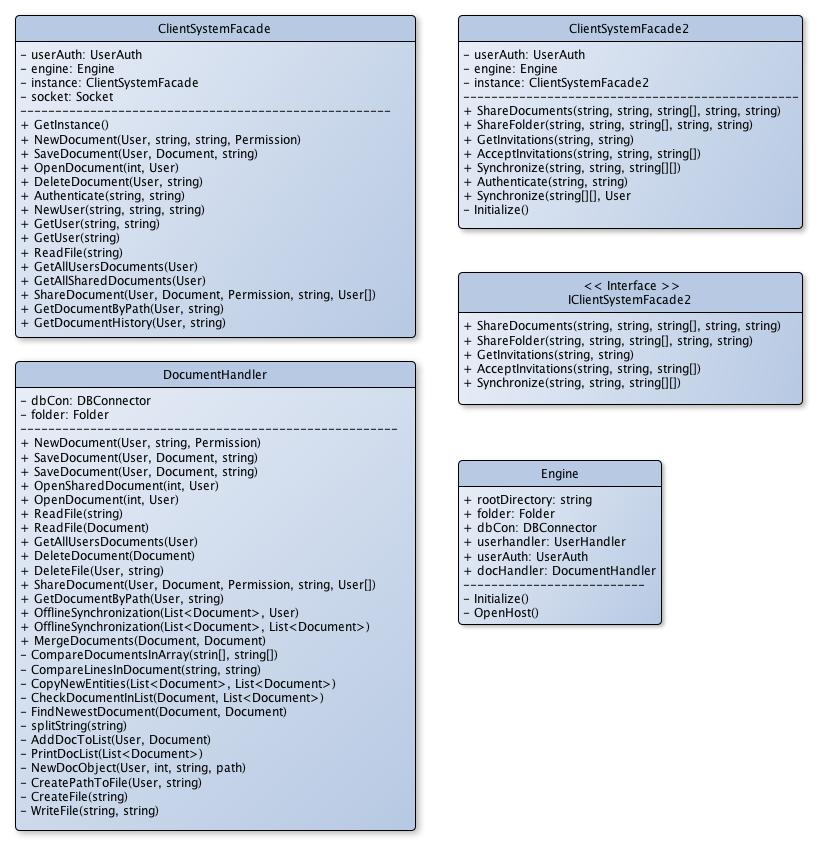
\includegraphics[width=300px]{images/ServerClassDiagram1of2.jpg}
    	\caption{Server class diagram}
\end{figure}

\begin{figure}[H]
  		\centering
    	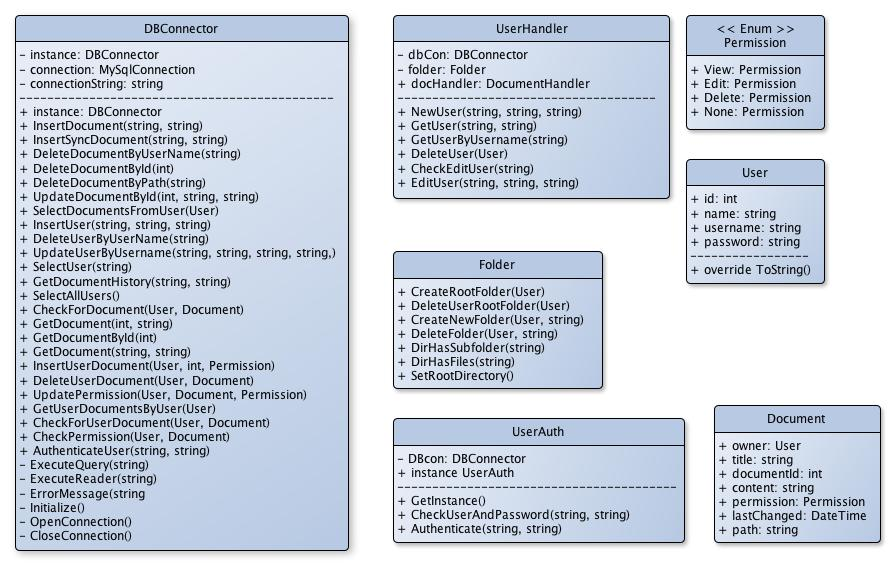
\includegraphics[width=300px]{images/ServerClassDiagram2of2.jpg}
    	\caption{Server class diagram}
\end{figure}

\begin{figure}[H]
  		\centering
    	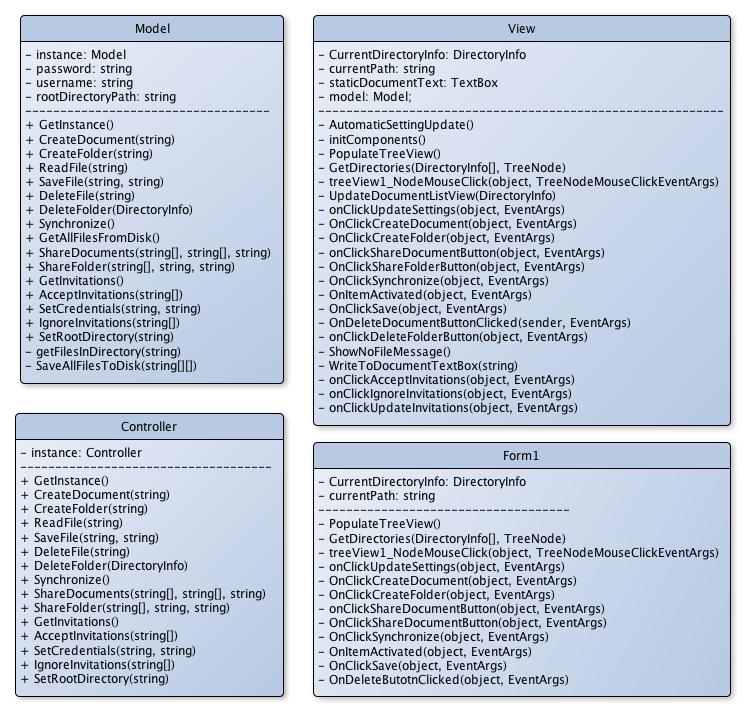
\includegraphics[width=300px]{images/StandAloneClient_CompleteClassDiagram.jpg}
    	\caption{StandAlone Client class diagram}
\end{figure}

\begin{figure}[H]
  		\centering
    	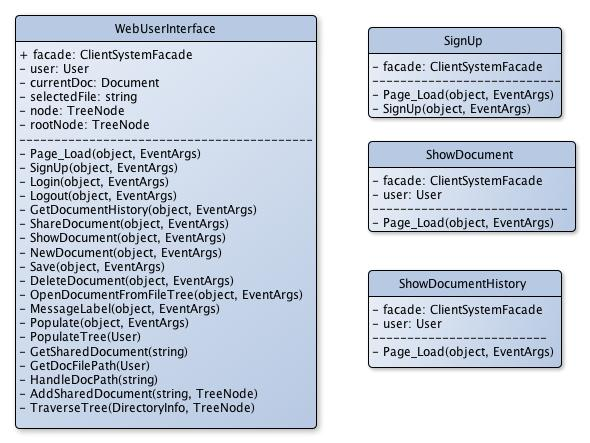
\includegraphics[width=300px]{images/WebUICompleteClassDiagram.jpg}
    	\caption{WebUI class diagram}
\end{figure}

\begin{figure}[H]
  		\centering
    	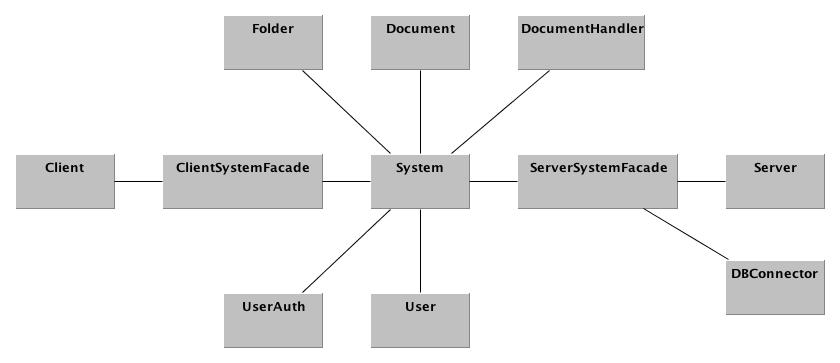
\includegraphics[width=300px]{images/ClassDiagramFirstDraft.jpg}
    	\caption{Old version of class diagram}
\end{figure}

\section{Package diagram}
\begin{figure}[H]
  		\centering
    	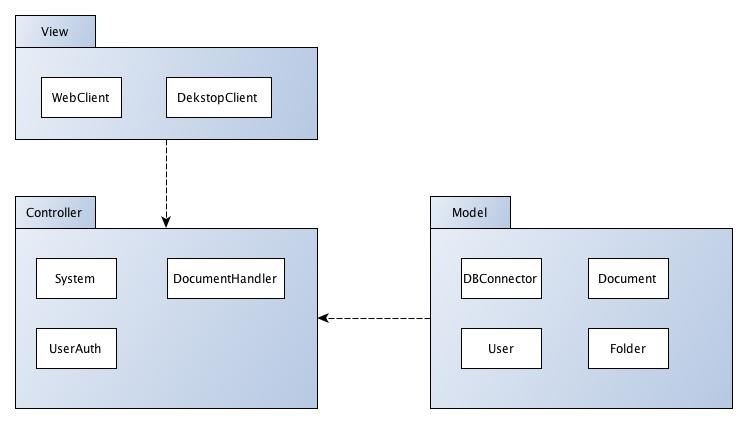
\includegraphics[width=300px]{images/PackageDiagramOverview.jpg}
    	\caption{System package diagram}
\end{figure}

\section{Sprint tables}

\begin{figure}[H]
  		\centering
    	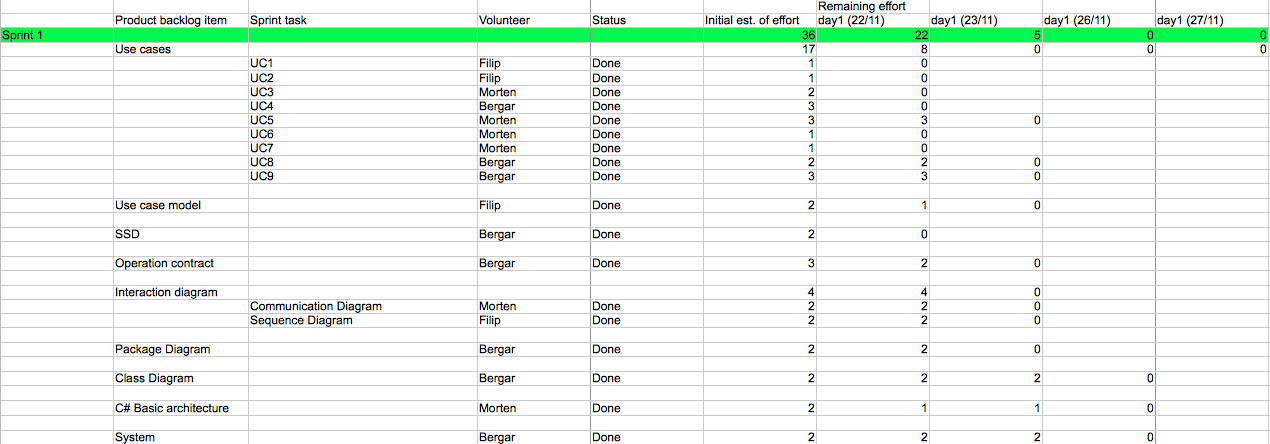
\includegraphics[width=300px]{images/Sprint1_Table.png}
    	\caption{1. Sprint table}
\end{figure}

\begin{figure}[H]
  		\centering
    	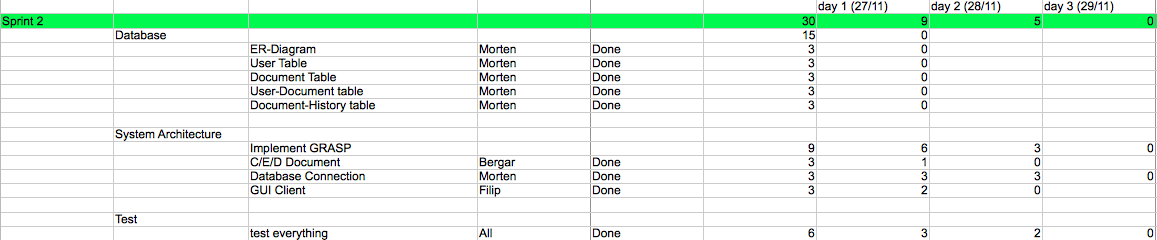
\includegraphics[width=300px]{images/Sprint2_Table.png}
    	\caption{2. Sprint table}
\end{figure}

\begin{figure}[H]
  		\centering
    	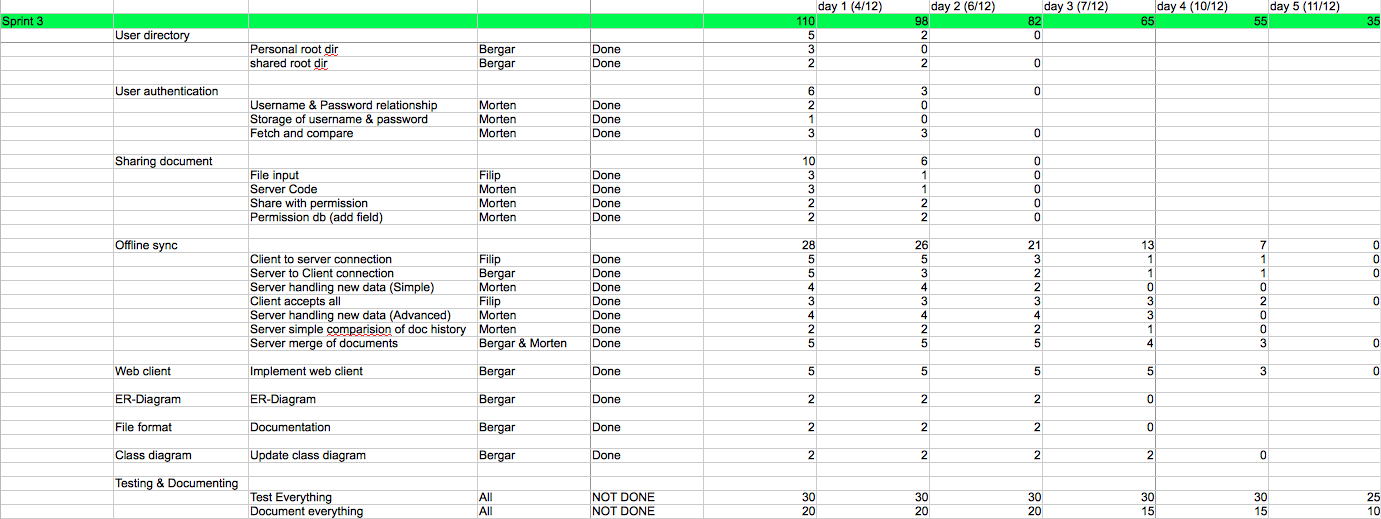
\includegraphics[width=300px]{images/Sprint3_Table.png}
    	\caption{3. Sprint table}
\end{figure}

\section{Use Cases}

% Use case 1
\fbox{\begin{minipage}{\columnwidth}
		\textbf{Use case UC1: Create new document} \\ 
		\textbf{Scope:} Slice-of-pie application \\
		\textbf{Level:} User goal \\
		\textbf{Primary actor:} Regular user \\
		\textbf{Stakeholders and Interests: } \\
		- Regular user: Wants to create a new document without any complications. \\
		\textbf{Preconditions:} none. \\
		\textbf{Postconditions:} The document will be created\\
		
		\textbf{Basic flow:} 
		\begin{enumerate}
			\item The user needs a document that can be shared with others.
			\item The user chooses a client program (web or desktop client).
			\item The user presses the "New Document" button.
			\item The client presents a dialogue box.
			\item The user types information about the document and press OK.
			\item The client sends a request to the server and the document gets stored by the server.
			\item The client displays the document for the user.
		\end{enumerate} 
		\textbf{Extensions:}
			\begin{enumerate}
				\item[6.]  The server is not responding \\
				\begin{enumerate}
					\item The document is saved locally.
					\item The client requests the server in regular intervals to see if it has recovered.
				\end{enumerate}
			\end{enumerate}
		\textbf{Special requirements:} \\
		- The document should be displayed properly on any devices such as smart phones and tablets. \\
\end{minipage}}

% Use case 2
\fbox{\begin{minipage}{\columnwidth}
		\textbf{Use case UC2: Edit document} \\ 
		\textbf{Scope:} Slice-of-pie application \\
		\textbf{Level:} User goal \\
		\textbf{Primary actor:} Regular user \\
		\textbf{Preconditions:} A document must have been created \\
		\textbf{Postconditions:} The document must be edited the way the user desires and the change must be recorded by the server too\\
		
		\textbf{Basic flow:} 
		\begin{enumerate}
			\item The user opens a document.
			\item The user edits the content of the document.
			\item The client sends a request to the server.
			\item The document is changed on the server.
		\end{enumerate} 
		\textbf{Extensions:}
			\begin{enumerate}
				\item[3.]  The server is not responding \\
				\begin{enumerate}
					\item The document is saved locally.
					\item The client requests the server in regular intervals to see if it has recovered.
				\end{enumerate}
			\end{enumerate}
		\textbf{Special requirements:} \\
		- The document should be displayed properly on any devices such as smart phones and tablets. \\		
\end{minipage}}

% Use case 3
\fbox{\begin{minipage}{\columnwidth}
		\textbf{Use case UC3: Delete document } \\ 
		\textbf{Scope:} Slice-of-pie application \\
		\textbf{Level:} User goal \\
		\textbf{Primary actor:} Regular user \\
		\textbf{Preconditions:} A document must have been created. The user trying to delete a document must have sufficient rights to delete selected document \\
		\textbf{Postconditions:} The document is now deleted from the users local repository, and will be deleted when user commits \\
		
		\textbf{Basic flow:} 
			\begin{enumerate}
			\item The user selects a document
			\item The user tries to delete the document 3. The client sends a request to the server 
			\item Server checks for authentication
			\item Document is deleted
			\end{enumerate}
		\textbf{Extensions:}
			\begin{enumerate}
			\item[3.] The server is not responding
			\begin{itemize}
			\item The document is saved locally
			\item The client requests the server in regular intervals to see if it has recovered			
			\end{itemize}
			\item[4.] The user lacks the right to delete the selected document
			\begin{itemize}
			\item User is told that he has not got the rights to delete selected document
			\end{itemize} 
			\end{enumerate}
		\textbf{Special requirements:} \\
\end{minipage}}	

% Use case 4
\fbox{\begin{minipage}{\columnwidth}
		\textbf{Use case UC4: Merging documents (Resolve conflict)} \\ 
		\textbf{Scope:} Slice of Pie application\\
		\textbf{Level:}  User goal\\
		\textbf{Primary actor:} Regular user\\
		\textbf{Preconditions:} A document must exist on the server and another (edited) version of the same document must exist on the stand-alone client\\
		\textbf{Postconditions:} Both versions (client and server) must have matching content\\
		
		\textbf{Basic flow:} 
		\begin{enumerate}
		\item The user opens an existing document on the client.
		\item The user edits the document and saves the lates changes.
		\item The stand-alone client and the server are synchronized.
		\item Both documents merge and contain both the original and the new content.
		\end{enumerate}
		\textbf{Extensions:} 
		\begin{enumerate}
		\item[*4.] There is a conflict when merging the documents.
		\begin{enumerate}
		\item The user resolves the conflict manually by editing the document.
		\item The user synchronizes again.
		\end{enumerate}				
		\end{enumerate}
		\textbf{Special requirements:} \\
\end{minipage}}

% Use case 5
\fbox{\begin{minipage}{\columnwidth}
		\textbf{Use case UC5: Offline synchronization} \\ 
		\textbf{Scope:} Slice-of-pie application \\
		\textbf{Level:} User goal \\
		\textbf{Primary actor:} Regular user \\
		\textbf{Preconditions:} User must be logged in. Client must be connected to the server. \\
		\textbf{Postconditions:} The users offline repository will be synchronized with his online repository \\
		
		\textbf{Basic flow:} \\
		\begin{enumerate}
		\item The user selects offline synchronization
		\item The client sends a request to the server.
		\item The server copies the user's online repository and sends it to the client
		\item The client sends verification upon receiving the documents
		\end{enumerate}
		\textbf{Extensions:} \\
		\begin{enumerate}
		\item[2.] The server is not responding
			\begin{itemize}
			\item The user gets an error message (no connection)
			\end{itemize}
		\item[4.] The server is not responding
			\begin{itemize}
			\item The client tries to re-establish a connection to the server at regular intervals, and then sends the verification.
			\end{itemize}
		\end{enumerate}
		\textbf{Special requirements:} \\
\end{minipage}}

% Use case 6
\fbox{\begin{minipage}{\columnwidth}
		\textbf{Use case UC6: Create new folder} \\ 
		\textbf{Scope:} Slice-of-pie application\\
		\textbf{Level:} User goal\\
		\textbf{Primary actor:} Regular user\\
		\textbf{Preconditions:} none.\\
		\textbf{Postconditions:} The folder will have been created\\
		
		\textbf{Basic flow:} 
		\begin{enumerate}
			\item User clicks on "create new folder" button
			\item User fills in valid folder information and clicks "OK"
			\item Client sends a request to server and server stores the folder
			\item Client displays the new folder
		\end{enumerate}
		\textbf{Extensions:} 
		\begin{enumerate}
			\item[2.] Information is not valid
			\begin{enumerate}
				\item User gets an error message describing what information is invalid
			\end{enumerate}
			\item[3.] Server does not respond
			\begin{enumerate}
				\item folder is stored locally
				\item The client requests the server in regular intervals to see if it has recovered, then resends the request to create a folder.
			\end{enumerate}
		\end{enumerate}
		\textbf{Special requirements:} \\
\end{minipage}}

% Use case 7
\fbox{\begin{minipage}{\columnwidth}
		\textbf{Use case UC7: Create new project} \\ 
		\textbf{Scope:} Slice-of-pie application\\
		\textbf{Level:}  User goal\\
		\textbf{Primary actor:} Regular user\\
		\textbf{Preconditions:} none.\\
		\textbf{Postconditions:} a Project will have been created\\
		
		\textbf{Basic flow:} \begin{enumerate}
			\item User clicks on "Create New Project" button
			\item User fills in valid Project information and clicks "OK"
			\item Client sends a request to server and server stores the Project
			\item Client displays the new folder
		\end{enumerate}
		\textbf{Extensions:} 
		\begin{enumerate}
			\item[2.] Information is not valid
			\begin{enumerate}
				\item User gets an error message describing what information is invalid
			\end{enumerate}
			\item[3.] Server does not respond
			\begin{enumerate}
				\item Project is stored locally
				\item The client requests the server in regular intervals to see if it has recovered, then resends the request to create a Project.
			\end{enumerate}
		\end{enumerate}
		\textbf{Special requirements:} \\
\end{minipage}}

% Use case 8
\fbox{\begin{minipage}{\columnwidth}
		\textbf{Use case UC8: View old version of document} \\ 
		\textbf{Scope:} Slice of Pie application\\
		\textbf{Level:} User goal\\
		\textbf{Primary actor:} Regular user \\
		\textbf{Preconditions:} A document with multiple changes must exist \\
		\textbf{Postconditions:} None\\		
		\textbf{Basic flow:} 
		\begin{enumerate}
		\item A user wants to see an overview of all changes made to a document.
		\item User opens a document.
		\item User presses a button and is presented with a list of all changes made to the specific document.
		\end{enumerate}
		\textbf{Extensions:} \\
		\textbf{Special requirements:} \\
\end{minipage}}

% Use case 9
\fbox{\begin{minipage}{\columnwidth}
		\textbf{Use case UC9:} Share document \\
		\textbf{Scope:} Slice of Pie application \\
		\textbf{Level:}  User goal\\
		\textbf{Primary actor:} Regular user\\
		\textbf{Preconditions:} A document must be created in the system and at least two users must be registered.\\
		\textbf{Postconditions:} The document is shared between two (or more) users.\\
		
		\textbf{Basic flow:} 
		\begin{enumerate}
		\item The users creates a new document or opens an existing one.
		\item The user selects which users he wants to share the document with.
		\item The user shares the document with the selected user(s).
		\end{enumerate}
		\textbf{Extensions:} \\
		\textbf{Special requirements:} \\
\end{minipage}}

% Use case 10
\fbox{\begin{minipage}{\columnwidth}
		\textbf{Use case UC10: Log in} \\ 
		\textbf{Scope:} Slice of Pie application\\
		\textbf{Level:}  User goal\\
		\textbf{Primary actor:} Regular user\\
		\textbf{Preconditions:} User must be registered in the system \emph{(see "extensions *2").}\\
		\textbf{Postconditions:} User is logged into the system.\\
		
		\textbf{Basic flow:} \\
		\begin{enumerate}
			\item When the user starts the system (web client or stand-alone client) he's prompted with a login screen.
			\item User must log in by typing username and password.
			\item System checks if information matches what is stored in the system.
			\item User is logged into the system.
		\end{enumerate}
		\textbf{Extensions:} \\
		\begin{enumerate}
			\item[*2.] User is not registered in the system.
		\begin{enumerate}
			\item User is prompted with a sign up screen (web-client only).
			\item User fills out required information for signing up.
		\end{enumerate}
			\item[*4.] Username and password are rejected.
		\begin{enumerate}
			\item User gets an error message on the screen saying that the username and password don't match the system.
			\item User gets prompted back to the login screen.
		\end{enumerate}
		\end{enumerate}
		\textbf{Special requirements:} \\
\end{minipage}}






\end{document}